\section{Fundamentals\label{chap:fundamentals}}

To understand how \lare{} works a few technologies are required to know about.
\html{}, the markup language which is used to create \webPage{}s, is the first technology which is mentioned in this chapter.
Afterwards \httpRequest{}s are presented as the fundamental transfer protocol of the World Wide Web.
Dynamic content and synchronicity are the topics explained next, the problem addressed by \ajax{} and \singlePageApplication{}s, which are presented subsequently.
The History API, released in October 2014, is required by \lare{} and presented at the end of this chapter.

\subsection{\html{}\label{html}}
Hypertext Markup Language (\html{}) is the language which is used to create webpages.
It's specification is defined by the \gls{w3c}\footnote{http://www.w3.org/TR/html5/ (Accessed: June 24, 2015)}.
It allows to structure a web document semantically, but not to style it.
Similar to XML it consists of hierarchically structured tags.
Each tag may have attributes.
Allowed attributes are defined per tag, e.g. an anchor tag (<a>) may have an href attribute, which is not allowed on a div tag (<div>).
This href attribute defines where the anchor should lead to, when clicked on.
\\
Another type of attribute is the data attribute whose name starts with the string \enquote{data-} followed by at least one other character.
Those attributes are intended to store custom information, for which there are no more appropriate attributes or elements.
\\
There is a special attribute called \enquote{id} which defines the unique identifier of a tag.
Each value of it may not occur more than once on a \webPage{}.

\begin{figure}[H]
\centering
\includegraphics[width=13cm]{images/lare_html.pdf}
\caption[lare_html]{Sample HTML structure of a web application using \lare{}}
\label{fig:lare_html}
\end{figure}

\noindent{}Figure \ref{fig:lare_components} shows the rendered structure of a sample \webApplication{} which is used to demonstrate \lare{} and other techniques in this thesis.
An <div> tag with the ID site (blue) contains among others a container with the ID page(pink).
This contains the <div> tags with IDs tags\_headline(red) and content(green).
\\
The HTML to this structure can be similar to listing \ref{lst:example_html}. It stats with \emph{<!Doctype html>} which defines that this HTML document uses the HTML in the version 5.
Surrounding every code afterwards follows the \emph{<html>...</html>} tag.
\\
The \emph{<head>...</head>} part of a site, defines an area in the HTML document, which is not rendered directly but can be used to set a title of the \webPage{}, \emph{<meta>} keywords for crawlers or \emph{<link>} tags to include resources like Cascading Style Sheets(CSS) to style the document.
Additionally in this area JavaScript(JS) can be defined or included to gain more functionality in the user interface(UI).
\\
The \emph{<body>...</body>} part of a HTML document is the space where the content should be in.
This area is rendered and presented to the user.
In our case some div tags in the structure mentioned before are located here.

\begin{minipage}[c]{0.95\linewidth}
\begin{lstlisting}[caption=Sample HTML document, label=lst:example_html]
<!Doctype html>
<html>
<head>
  ...
</head>
<body>
    ...
    <div id="site">
        ...
        <div id="page">
            ...
            <div id="tags_headline"></div>
            ...
            <div id="content"></div>
            ...
        </div>
        ...
    </div>
    ...
</body>
</html>
\end{lstlisting}
\end{minipage}

\subsection{\httpRequest{}s\label{httpRequest}}
The World Wide Web has one main protocol to let \webBrowser{}s and \webServer{}s communicate, the Hypertext Transfer Protocol (\http{}), which is built on top of the Transmission Control Protocol (TCP).
TCP and so \httpRequest{}s always start with a handshake to establish a connection before data is transferred.
After this handshake, the client sends the request data to the \webServer{}.

\noindent{}This recognizes and interprets the request and if the requested resource is available, sends the according data back, otherwise it sends an error.
\WebApplication{}s typically render data out of a database into a \html{} template and sends it back as the response.
The browser receives this \webPage{} interprets and renders it.
Subsequently it sends \httpRequest{}s to receive the images, CSS and JS linked in this page.
\\
Figure \ref{fig:http_components} displays this request/response communication of a \webBrowser{} and a \webServer{} when requesting a \webPage{} initially.

\begin{figure}[H]
\centering
\includegraphics[height=7cm]{images/http.pdf}
\caption[http_components]{Component and communication diagram of \http{}}
\label{fig:http_components}
\end{figure}

\subsection{Dynamic content and synchronicity\label{synchronicity}}

Common \httpRequest{}s, which are described in \ref{httpRequest}, do not support asynchronous changes of content. As presented in fig. \ref{fig:http_components} the response of common \httpRequest{}s is always a full page, which replaces the previous one fully.

\begin{figure}[H]
\centering
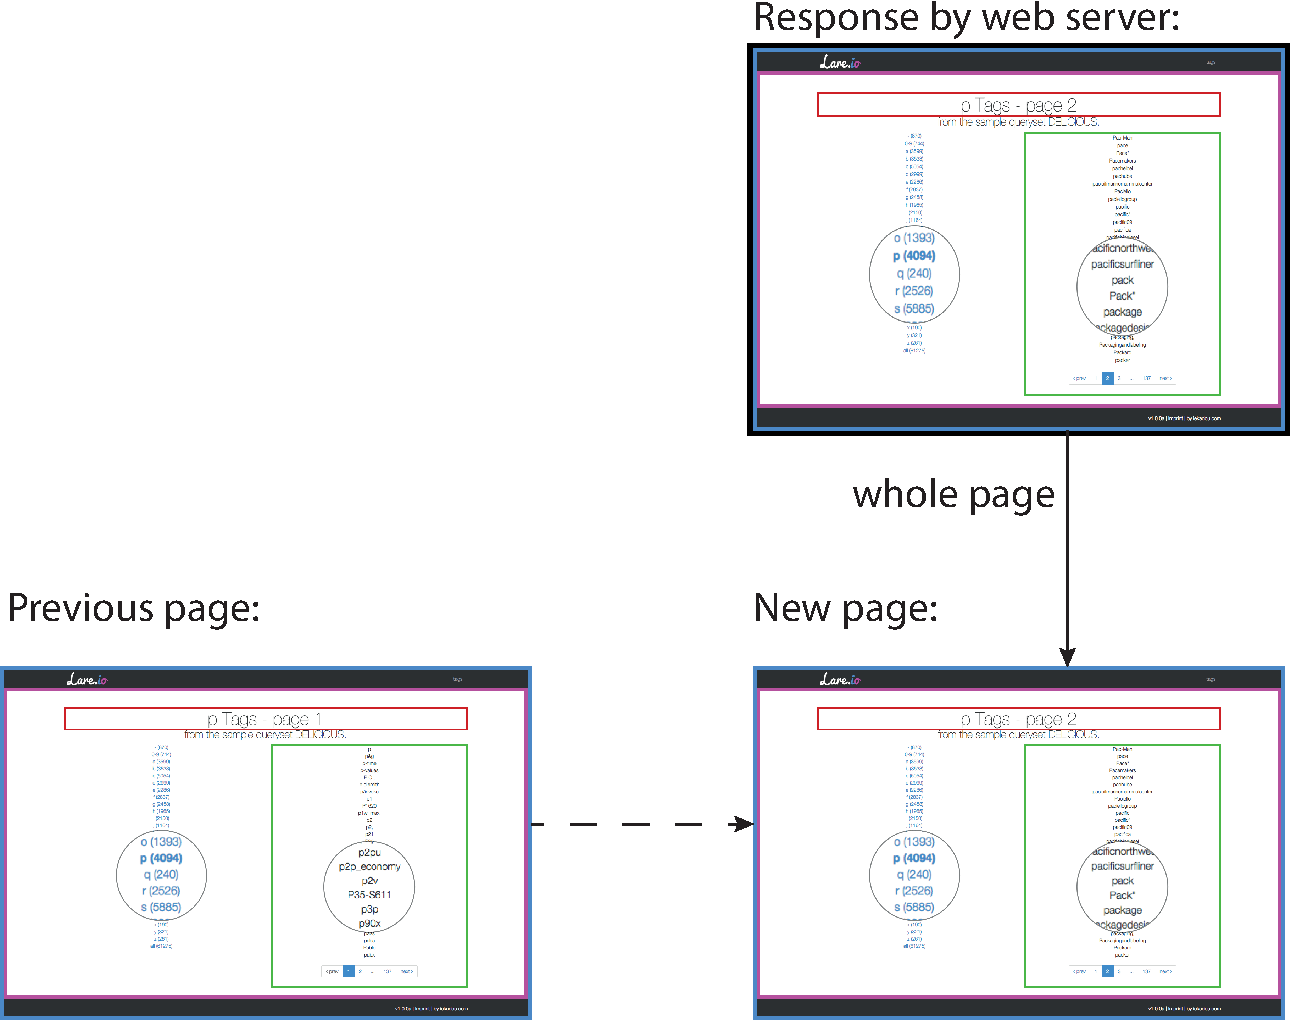
\includegraphics[width=12cm]{images/http_replacements.pdf}
\caption[ajax_replacements]{Content replacements by common \httpRequest{}s}
\label{fig:ajax_replacements}
\end{figure}

\noindent{}To retrieve new information the client has to request another full \webPage{}, including all resources and data which is necessary.
This makes this kind of \webSite{} \enquote{synchronous}.
Even if newer \http{} versions recommend asynchronous requests to retrieve resources, the HTML document itself still is synchronous. 
An \enquote{asynchronous} \webSite{} is able to change content \emph{dynamically} without having to load a whole new page.
\ajax{}, as shown in \ref{ajax}, is the most used technique for asynchronous \webSite{}s.
\\
Often mixed up with the term synchronicity is the expression dynamic content.
Dynamic content in \webSite{}s is content which is not statically saved on the \webServer{}, as static content is.
Typically it gets fetched via backend services.
A backend service can be a database or other sort of API to derive information from.
Often it changes too often to save it in the filesystem of the \webServer{}.
Other reasons for this type of content can be using a content management system, or depending on data which you can not influence and has to be changed by others.
\\
Dynamic content and static content can both be delivered in synchronous and asynchronous \webApplication{}s.


\subsection{\ajax{}\label{ajax}}
Asynchronous JavaScript and XML (\ajax{}) is a technology to implement dynamic \webPage{}s.
The JavaScript structure XMLHttpRequest (XHR) is used to make requests to a \webServer{} without loading a full new page.
The response then is interpreted by an \ajax{}-engine.

A normal \httpRequest{} by a browser forces requests always to be synchronous.
\ajax{} can improve that.
The data flow, shown in fig. \ref{fig:ajax_components}, is very similar to the normal browser behaviour, but is using a new component: the \enquote{\ajax{}-engine}.
The first request to a \webServer{} using \ajax{} is the complete same as one without \ajax{} with the exception, that one of the requested sources is a JavaScript, which instantiates a \ajax{}-engine.

\begin{figure}[H]
\centering 
\includegraphics[height=10cm]{images/ajax.pdf}
\caption[ajax_components]{Component and communication diagram of \ajax{}}
\label{fig:ajax_components}
\end{figure}

\noindent{}The following requests are handled by this \ajax{}-engine, allowing to asynchronously request content from the \webServer{}.
\ajax{} can request only small parts of a website, most of the time in XML or JSON format, interprets it and then only adds, replaces or appends old content with the newly received.
Figure \ref{fig:ajax_replacements} shows that only one part of a \webPage{} is responded and replaced, instead of the whole page in \httpRequest{}s.

\begin{figure}[H]
\centering
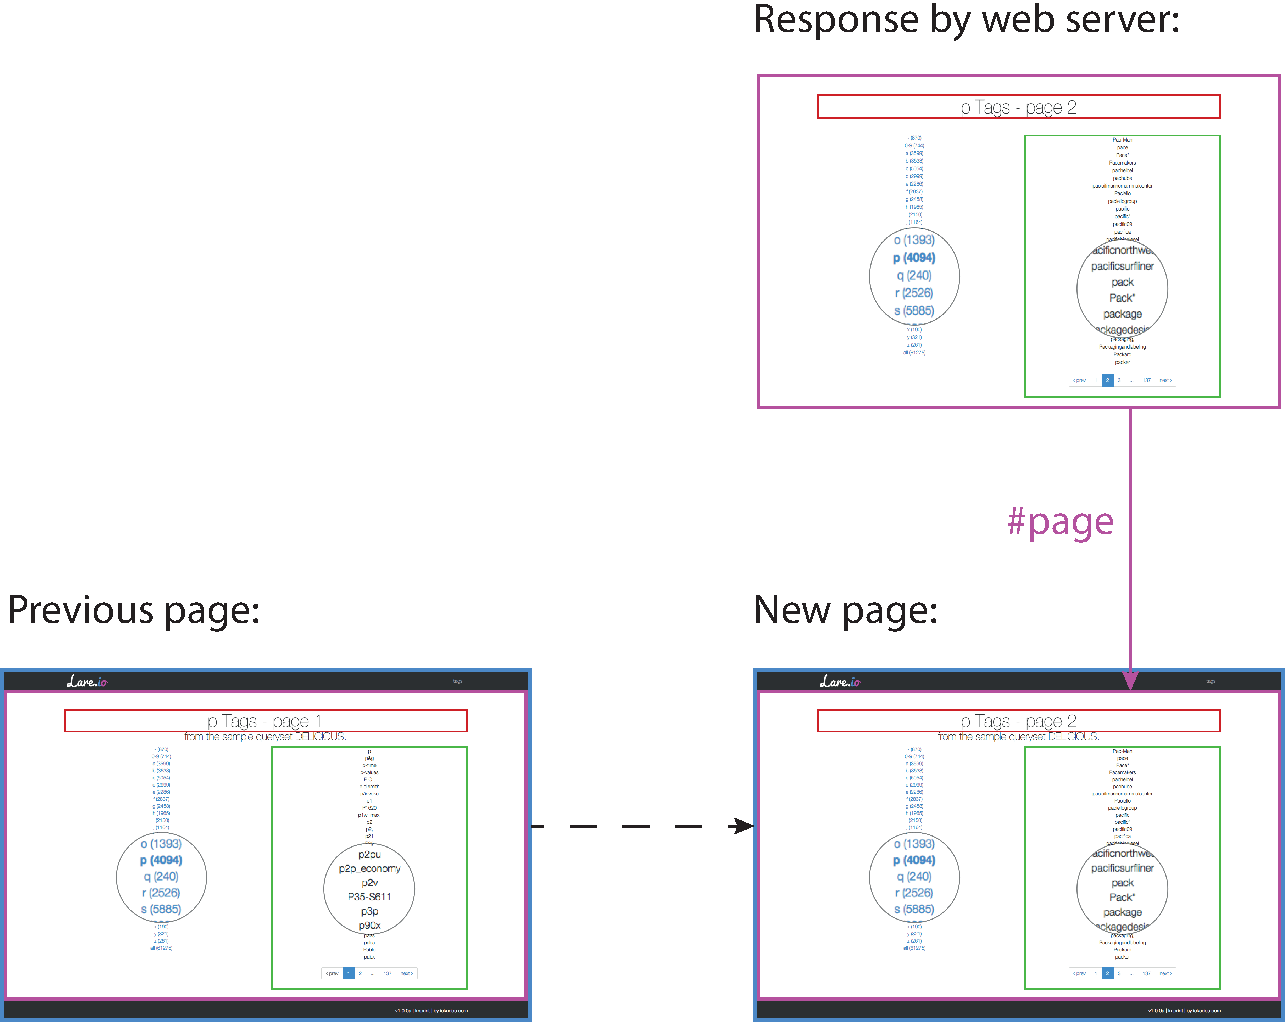
\includegraphics[width=12cm]{images/ajax_replacements.pdf}
\caption[ajax_replacements]{Content replacements by \ajax{}}
\label{fig:ajax_replacements}
\end{figure}

\subsection{\SinglePageApplication{}s\label{singlePageApplication}}
A \singlePageApplication{} (SPA) is a \webApplication{} or \webSite{} that only needs one full \webPage{} load.
Beside this there is no \webPage{} loaded completely at any point in the process anymore.
Often content changes are made asynchronous and dynamically by \ajax{} in response to user actions.
A disadvantage of a lot of \singlePageApplication{}s is the lack of browser history support.
When changing the content the browser does not interpret it as a new page, but only changed content.
This leads into a missing functionality of forward- and back-buttons in browsers.
\\
Additionally a problem of SPAs is, that it has a huge impact on search engine optimization (SEO).
The \webPage{} is often requested through multiple requests and brought together inside the browser. Often a \webSite{} is also not structured into different URLs.
Those facts make it hard for a search engines and other crawlers to discover it.

\subsection{History API}
The History API is part of the HTML5 specification by \gls{w3c}.
It describes the API for an History object which is part of the session history.
This session history enables functionality like the back and forward buttons on browsers.
Defined as a list of session history entries, it represents the browsing history.
A session history entry may be a URL or a state object and may have additional information.
\\
It is possible to influence this list via the window.history.pushState(data, title[, url]) method, which allows to add a new state into this list.
This also effects the browser's navigation bar, which gains the possibility for users to share or bookmark a \webPage{}.
\\